La cartographie interactive permet une éditorialisation des données selon des paramètres essentiellement géographiques, nous l’avons vu, même si d’autres filtres viennent la compléter et l’enrichir. Dans le cadre de mon stage, il m’a semblé ne pas pouvoir me restreindre à cette seule \indexmot{visualisation}. L’exploration des résultats des analyses m’a convaincu que, dans le cadre d’une recherche sur les matériaux et les couleurs des enluminures, la \indexmot{chronologie} est tout aussi importante que la \indexmot{géographie}. Ainsi, je crois que deux œuvres créées à des époques très différentes dans la même région peuvent avoir peu de points communs~; là où des enluminures réalisées à la même époque, mais dans des régions différentes, peuvent parfois révéler des similitudes significatives dans leurs analyses. Il s’agit donc de proposer une interface interactive qui repose non plus sur une interaction entre une \indexmot{géographie} et des mots-clefs, mais entre ces derniers et une \indexmot{chronologie}.\par
Le programme de recherche \enquote{La couleur~: artefacts, matière et cognition} présente deux atouts majeurs pour une valorisation scientifique~: la richesse tant qualitative que quantitative des analyses menées et la numérisation complète des manuscrits étudiés. Je crois que cette dernière doit être davantage mise en avant dans la conception d’une nouvelle \indexmot{visualisation}. En d’autres termes, l'exploration des données doit permettre une plus grande appréciation des enluminures par l'utilisateur, plutôt que de se focaliser uniquement sur les données, parfois un peu arides. La \indexmot{visualisation} doit être à la fois chronologique et visuelle, et ce sont ces raisons qui m’ont conduit à m’intéresser au projet \textit{\indexmot{VIKUS} Viewer}.\newpage

\section{\indexmot{VIKUS} Viewer~: un système de \indexmot{visualisation} web avancé}

Christopher Pietsch, le principal développeur du projet, présente \indexmot{VIKUS} Viewer comme un système de \indexmot{visualisation} web avancé qui permet d'explorer des collections culturelles à travers des aspects thématiques et temporels\footcite{university_of_applied_sciences_potsdam_vikus_nodate}. Le logiciel peut organiser des milliers d'artefacts culturels sur une toile dynamique. Il offre une exploration, simple d’utilisation, des motifs thématiques et temporels de grandes collections, tout en offrant un accès rapide à des images en haute résolution. Il appartient au projet \textit{Visualisierung kultureller Sammlungen}, qui a vu le jour à l’Université des Sciences Appliquées de Potsdam dans le cadre d’une recherche interdisciplinaire financée de 2014 à 2017. Son objectif était d’étudier de nouvelles formes d'interfaces utilisateur graphiques pour soutenir l'exploration du patrimoine culturel numérique. Ce projet a abouti à plusieurs propositions de \indexmot{visualisation}s qui sont visibles sur sa page internet\footcite{university_of_applied_sciences_potsdam_visualizing_nodate}.\par
Actuellement, \indexmot{VIKUS} Viewer est utilisé pour visualiser quelques collections, notamment les dessins de Frédéric-Guillaume IV de Prusse \footnote{https://vikusviewer.fh-potsdam.de/fw4/}, la bibliothèque de Johann Wolfgang von Goethe \footnote{https://vikusviewer.fh-potsdam.de/goethe/}, les pamphlets de la guerre de Sept Ans\footnote{https://vikusviewer.fh-potsdam.de/recs/}, les dessins et peintures de Vincent van Gogh\footnote{https://vikusviewer.fh-potsdam.de/vangogh/} ou encore les pancartes de la Marche des femmes de Boston en 2017\footnote{https://vikusviewer.fh-potsdam.de/artofthemarch/}​. À ma connaissance, il n’y a pas encore d’utilisation connue de \indexmot{VIKUS} Viewer en France. Avec le dépôt Github que j’ai réalisé au cours de ce stage, la \indexmot{Bibliothèque nationale de France} est probablement l’une des premières à le faire\footnote{https://github.com/TheoBurnel/vikus\_bnf.git}.\\\par
Le code derrière \indexmot{VIKUS} est librement accessible sur un dépôt Github\footnote{ https://github.com/cpietsch/vikus-viewer.git}~–~sous une licence MIT – qu’il suffit de cloner et de faire tourner sur un serveur web\footnote{Comme pour la bibliothèque \indexmot{Leaflet}, j’ai travaillé sur VSCode avec Live Server.}. Il est constitué de HTML, CSS et JS\footnote{Il faut ajouter les bibliothèques pixi.js et d3.js.}. Si la documentation est sommaire, les développeurs ont déposé des modèles pour l’élaboration des métadonnées qui peuvent être repris. Concernant la gestion des images, qu’il faut transformer, un lien vers un script est présent\footnote{https://github.com/cpietsch/vikus-viewer-script.git}. Ainsi, si le futur fichier \enquote{data}, qui contient les fichiers config.json, data.csv, timeline.csv et info.md, est réalisé selon les modèles préexistants en utilisant des transformations Python pour s’en approcher le plus possible~; les images, elles, sont traitées par un script fournit par les développeurs de \indexmot{VIKUS}. Elles sont préparées en texture et en feuilles de \enquote{sprites}, c’est-à-dire en une image qui contient plusieurs plus petites images.\par
Christopher Pietsch propose en complément à son code une vue alternative. Elle repose sur une mise en page t-SNE, basée sur la similitude de l'image. Un script crée un fichier tsne.csv qui contient un tri des images selon leur ressemblance. Cependant, l’essai que j’ai réalisé à partir d’un petit échantillon ne me semble pas suffisamment convaincant pour le proposer dans le cadre de ce stage. Je propose donc ici deux fonctionnalités de la visionneuse \indexmot{VIKUS}~: une articulation entre une \indexmot{chronologie} et des mots-clefs, ainsi qu’une \indexmot{visualisation} en haute résolution des feuillets avec un contenu explicatif. \newpage

\section{Éditorialiser avec Vikus}

\indexmot{VIKUS} Viewer rend accessible de grandes collections de documents historiques avec une interface visuelle dynamique et intuitive. Le nombre de feuillets à faire apparaître au sein de la \indexmot{visualisation} ne représente aucunement un obstacle, mais, bien au contraire, donne un sens supplémentaire au choix de ce logiciel. Plus le corpus est important, plus la \indexmot{visualisation} dynamique gagne en pertinence. Elle permet de quantifier et d’observer les déplacements des feuillets selon les variables retenues, qu’elles soient chronologiques ou par mots-clefs.\par
La capture d’écran ci-dessous représente l’évolution de la \indexmot{visualisation}, depuis son lancement par l’utilisateur, en l’absence de filtre, puis avec la sélection du matériau \enquote{oxyde de plomb}. Le déplacement des icônes, qui sont des images des feuillets, représente le résultat alors obtenu. L’évolution de la hauteur des colonnes traduit la sélectivité effectuée par le filtre.\par
\begin{figure}[H]
	\centering
	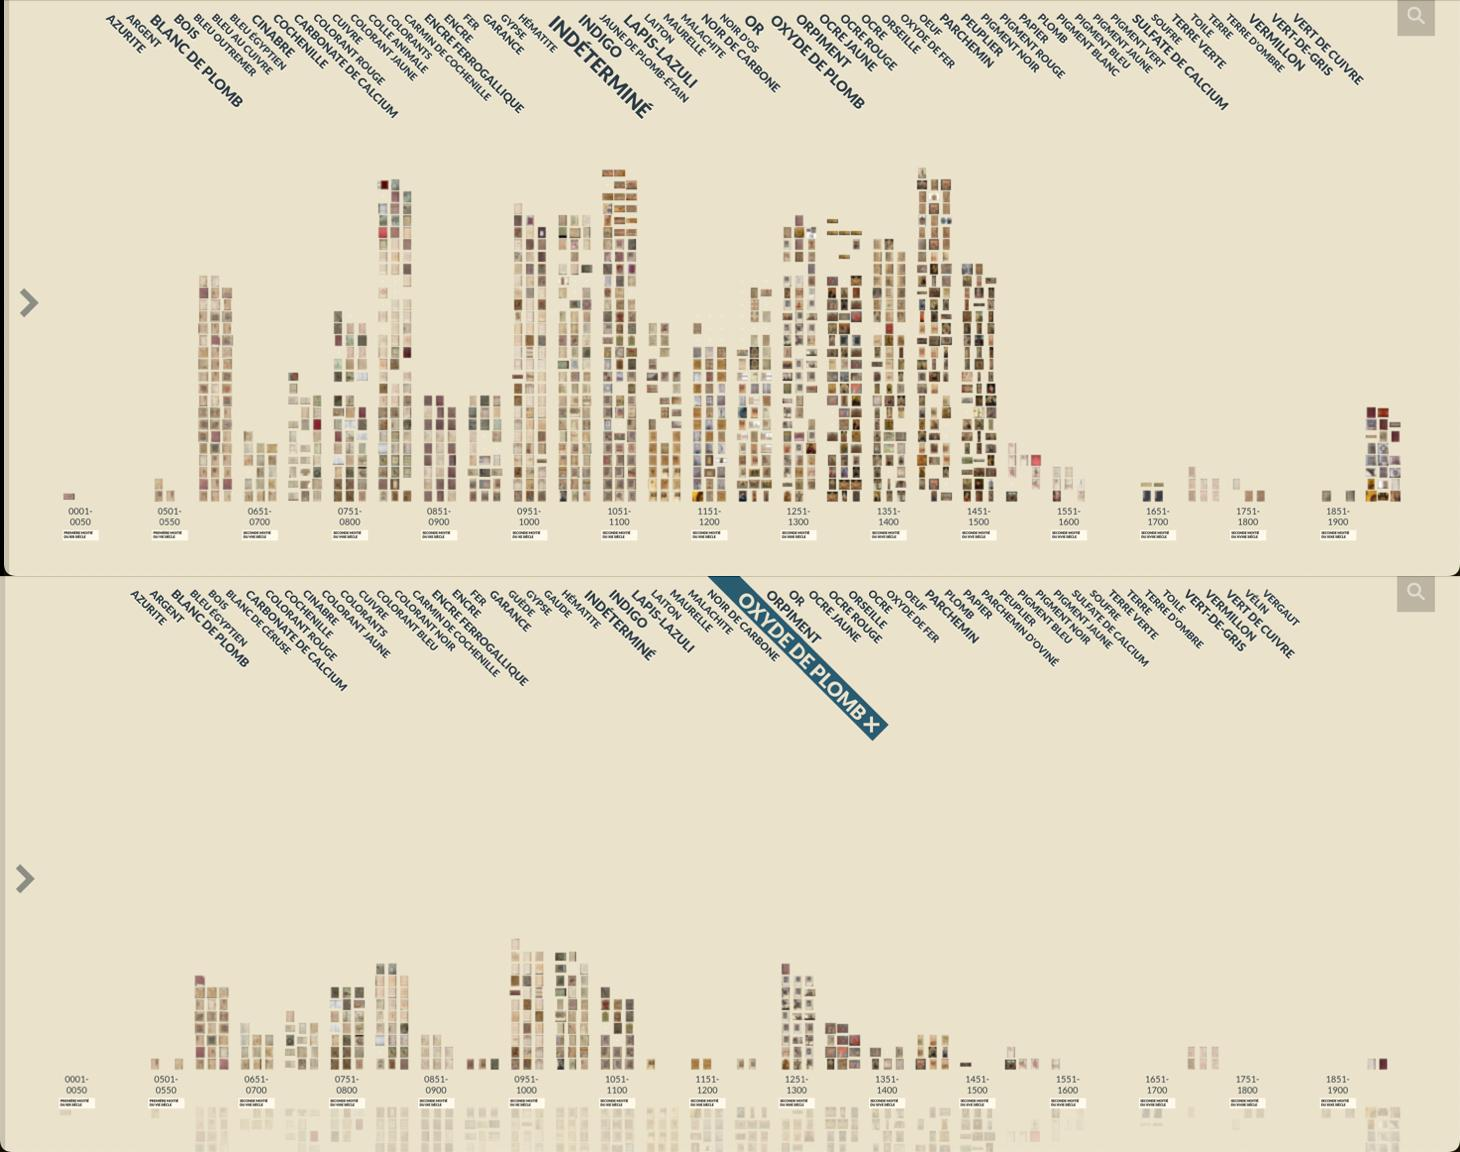
\includegraphics[width=\textwidth]{./textes/chap3/vikus-dyna.jpg}
	\caption{Déplacement d'icônes dans Vikus}
	\label{fig:info}
\end{figure}

Le filtrage repose sur deux paramètres, des séquences chronologiques et des thèmes spécifiques. Les données suivent une distribution temporelle dans \indexmot{VIKUS}. Cette \indexmot{chronologie} doit faciliter la compréhension d’un contexte historique et de tendances au fil du temps. La difficulté, pour un corpus comme le nôtre, réside dans la fragmentation et l’incertitude des datations. Les enluminures des manuscrits ne peuvent être que difficilement datées. Elles font bien souvent l’objet d’une estimation, d’une approximation chronologique afin de proposer un contexte historique vraisemblable. Parfois, l’ordre de grandeur est seulement de quelques années, parfois il est de plusieurs décennies. Dans une \indexmot{frise chronologique} classique, ces incertitudes sont contournées par la figuration de jauges, de segment qui indiquent les bornes de la datation. Une telle approche n’est pas possible sur \indexmot{VIKUS}. Les datations sont elles-mêmes des entités et pas seulement des valeurs. Elles ne peuvent pas se chevaucher ou se croiser. Chaque datation doit avoir une valeur unique et chaque feuillet doit avoir une seule datation. Dès lors, un certain arbitraire s’impose dans l’assignation d’un contexte de création à une enluminure.\par
L’autre difficulté réside dans le découpage de la \indexmot{chronologie}. Les feuillets apparaissent par colonne au-dessus de leur datation~: plus ces dernières seront nombreuses, plus les colonnes seront petites et peu lisibles~; moins les datations seront nombreuses, plus les résultats perdent en sens, diluant les mouvements artistiques dans de grandes ères historiques. Il me semble qu’une répartition par demi-siècle est, au regard du corpus, la meilleure division possible. Elle permet une \indexmot{visualisation} lisible et fluide, tout en n’élargissant pas exagérément les séquences chronologiques. Elle a, néanmoins, l’inconvénient de rapprocher artificiellement des productions séparées parfois de près de quatre décennies et d’en séparer d’autres proches de seulement quelques années. Ainsi, sur une même colonne, pourraient figurer des enluminures des années 1350 et 1390, mais elles seraient séparées de celles du début de la décennie 1400. Il y a là un biais propre à \indexmot{VIKUS} que je ne peux contourner. Néanmoins, la \indexmot{chronologie} de plus d’un millénaire sur laquelle reposent les analyses effectuées permet de lisser ce défaut, lorsque le regard est porté sur un temps long.\textit{Voir la figure 3.2.}\par
\begin{figure}[p]
	\centering
	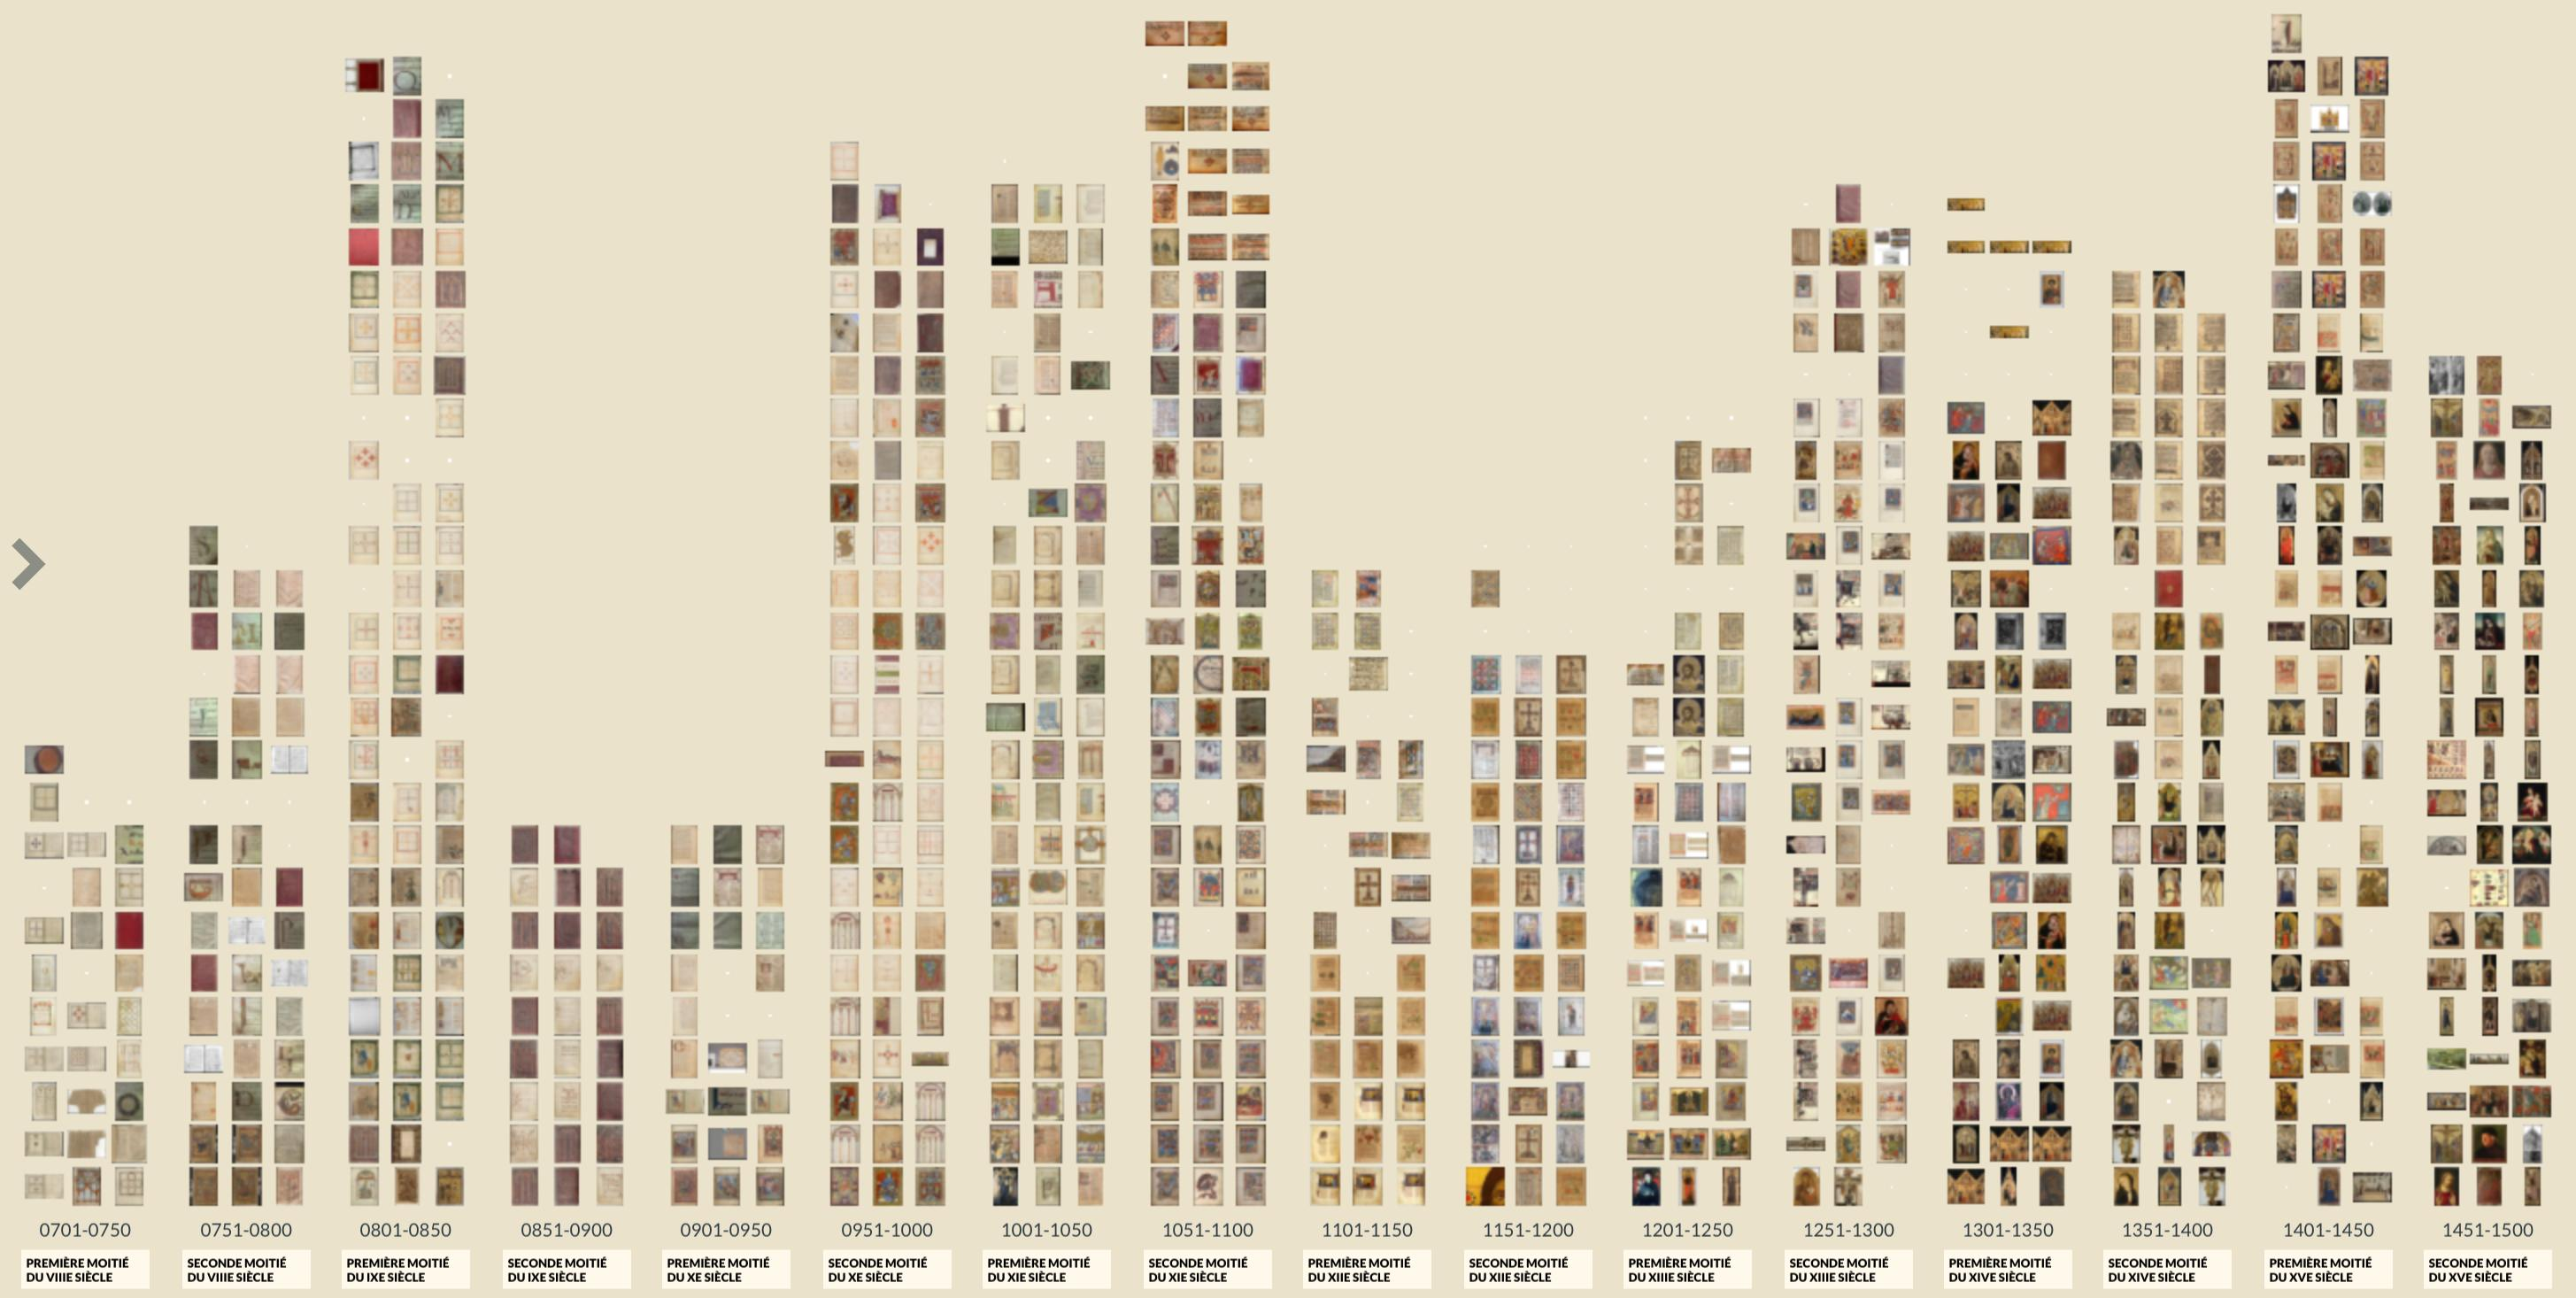
\includegraphics[width=\textwidth]{./textes/chap3/vikus-chrono.jpg}
	\caption{Les séquences chronologiques dans la frise}
	\label{fig:info}
\end{figure}

La seconde variable repose sur l’ontologie des matériaux. Comme pour la \indexmot{carte interactive}, le matériau est à nouveau le pivot des résultats obtenus. La navigation se fait à travers les mots-clefs, isolés et rangés alphabétiquement, présents dans la partie supérieure de la fenêtre. La taille de ces valeurs varie en fonction de leur occurrence~: si un matériau apparaît fréquemment dans le corpus, il aura une police supérieure à celle d’un autre plus rare. Le filtre par matériau proposé dans cette \indexmot{visualisation} permet de combiner les valeurs, ce qui n’est pas le cas sur la \indexmot{carte interactive}. La recherche s’affine et il est possible d’interroger la co-présence de matériaux au sein d’un même feuillet. Dans le cas ci-dessous, la première recherche est faite sur la seule présence de cochenille, puis elle se précise dans un second temps avec celle d’orseille. Le résultat obtenu est une \indexmot{visualisation} très précise sur leur usage commun à partir de la seconde moitié du Xe siècle et qui demeure rare dans le temps.\textit{Voir la figure 3.3.}\par
\begin{figure}[p]
	\centering
	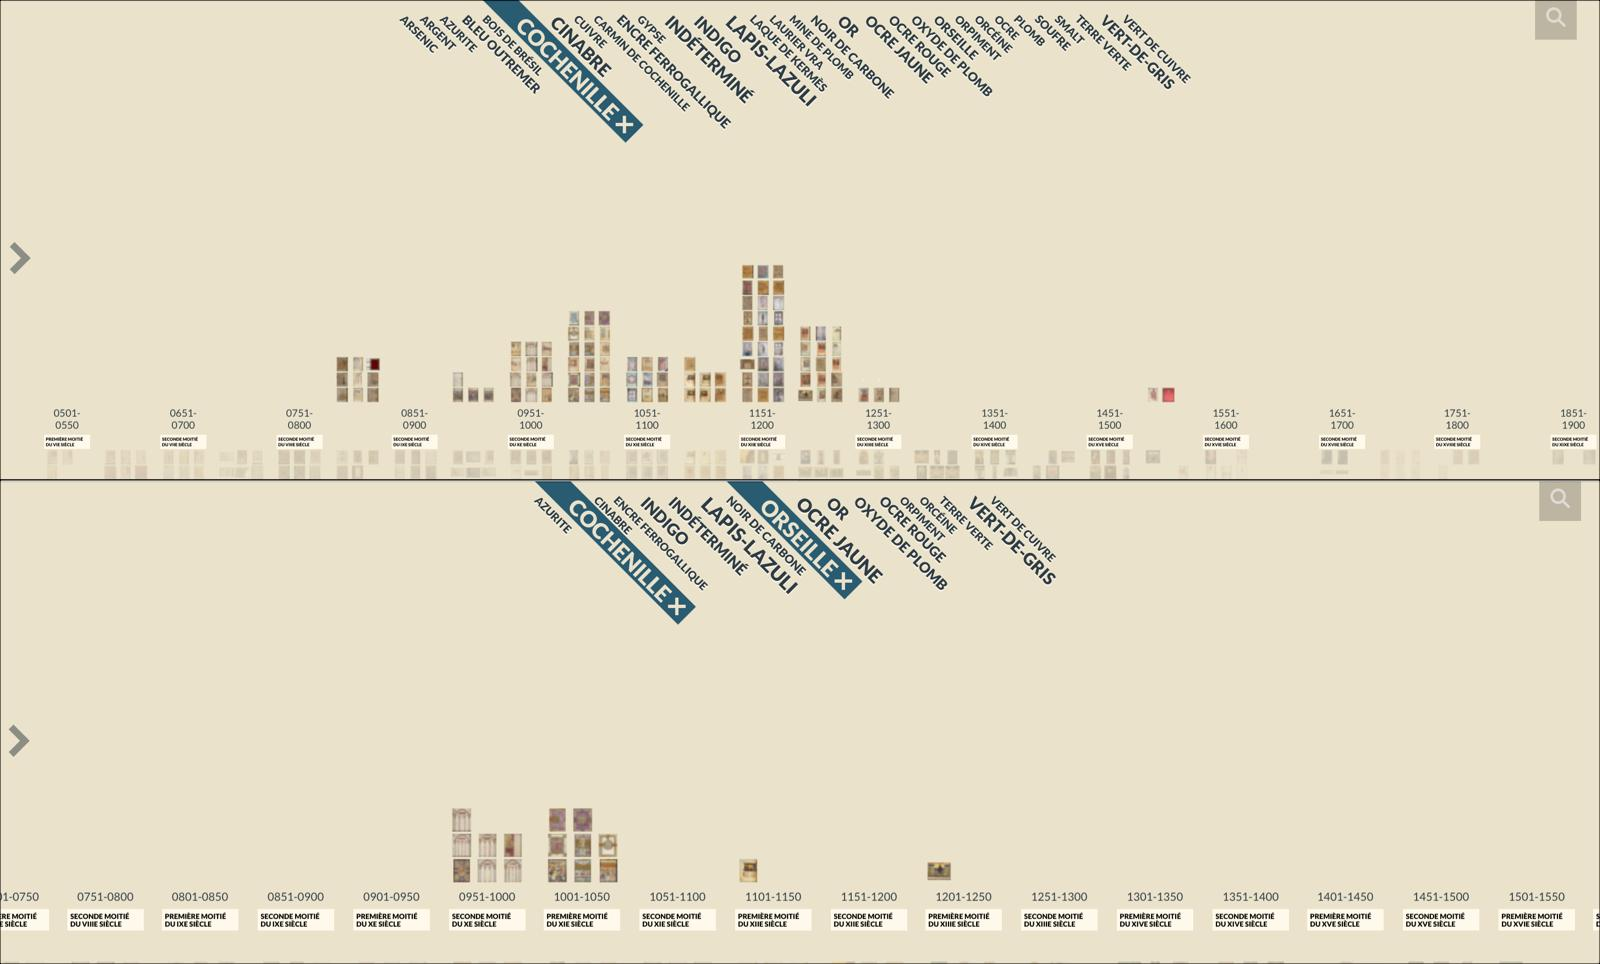
\includegraphics[width=\textwidth]{./textes/chap3/vikus-double.jpg}
	\caption{Co-présence de matériaux}
	\label{fig:info}
\end{figure}

Les \textit{artefacts}, comme les appelle Christopher Pietsch, qui sont traités par le logiciel, prennent l’apparence de l’image du feuillet. Elles se déplacent sur l’ensemble de l’interface selon le paramétrage du filtre. Avec un niveau de zoom suffisant ou avec un clic, l’interface fait apparaître une barre latérale à côté de l’image. Elle reprend les informations essentielles du feuillet. J’y fais figurer le titre de l’œuvre, les matériaux qui sont utilisés pour sa réalisation, les résultats des différentes analyses, son lieu de création ainsi que sa localisation actuelle. L’utilisateur a à sa disposition toutes les informations essentielles pour appréhender le manuscrit.\par

\begin{figure}[H]
	\centering
	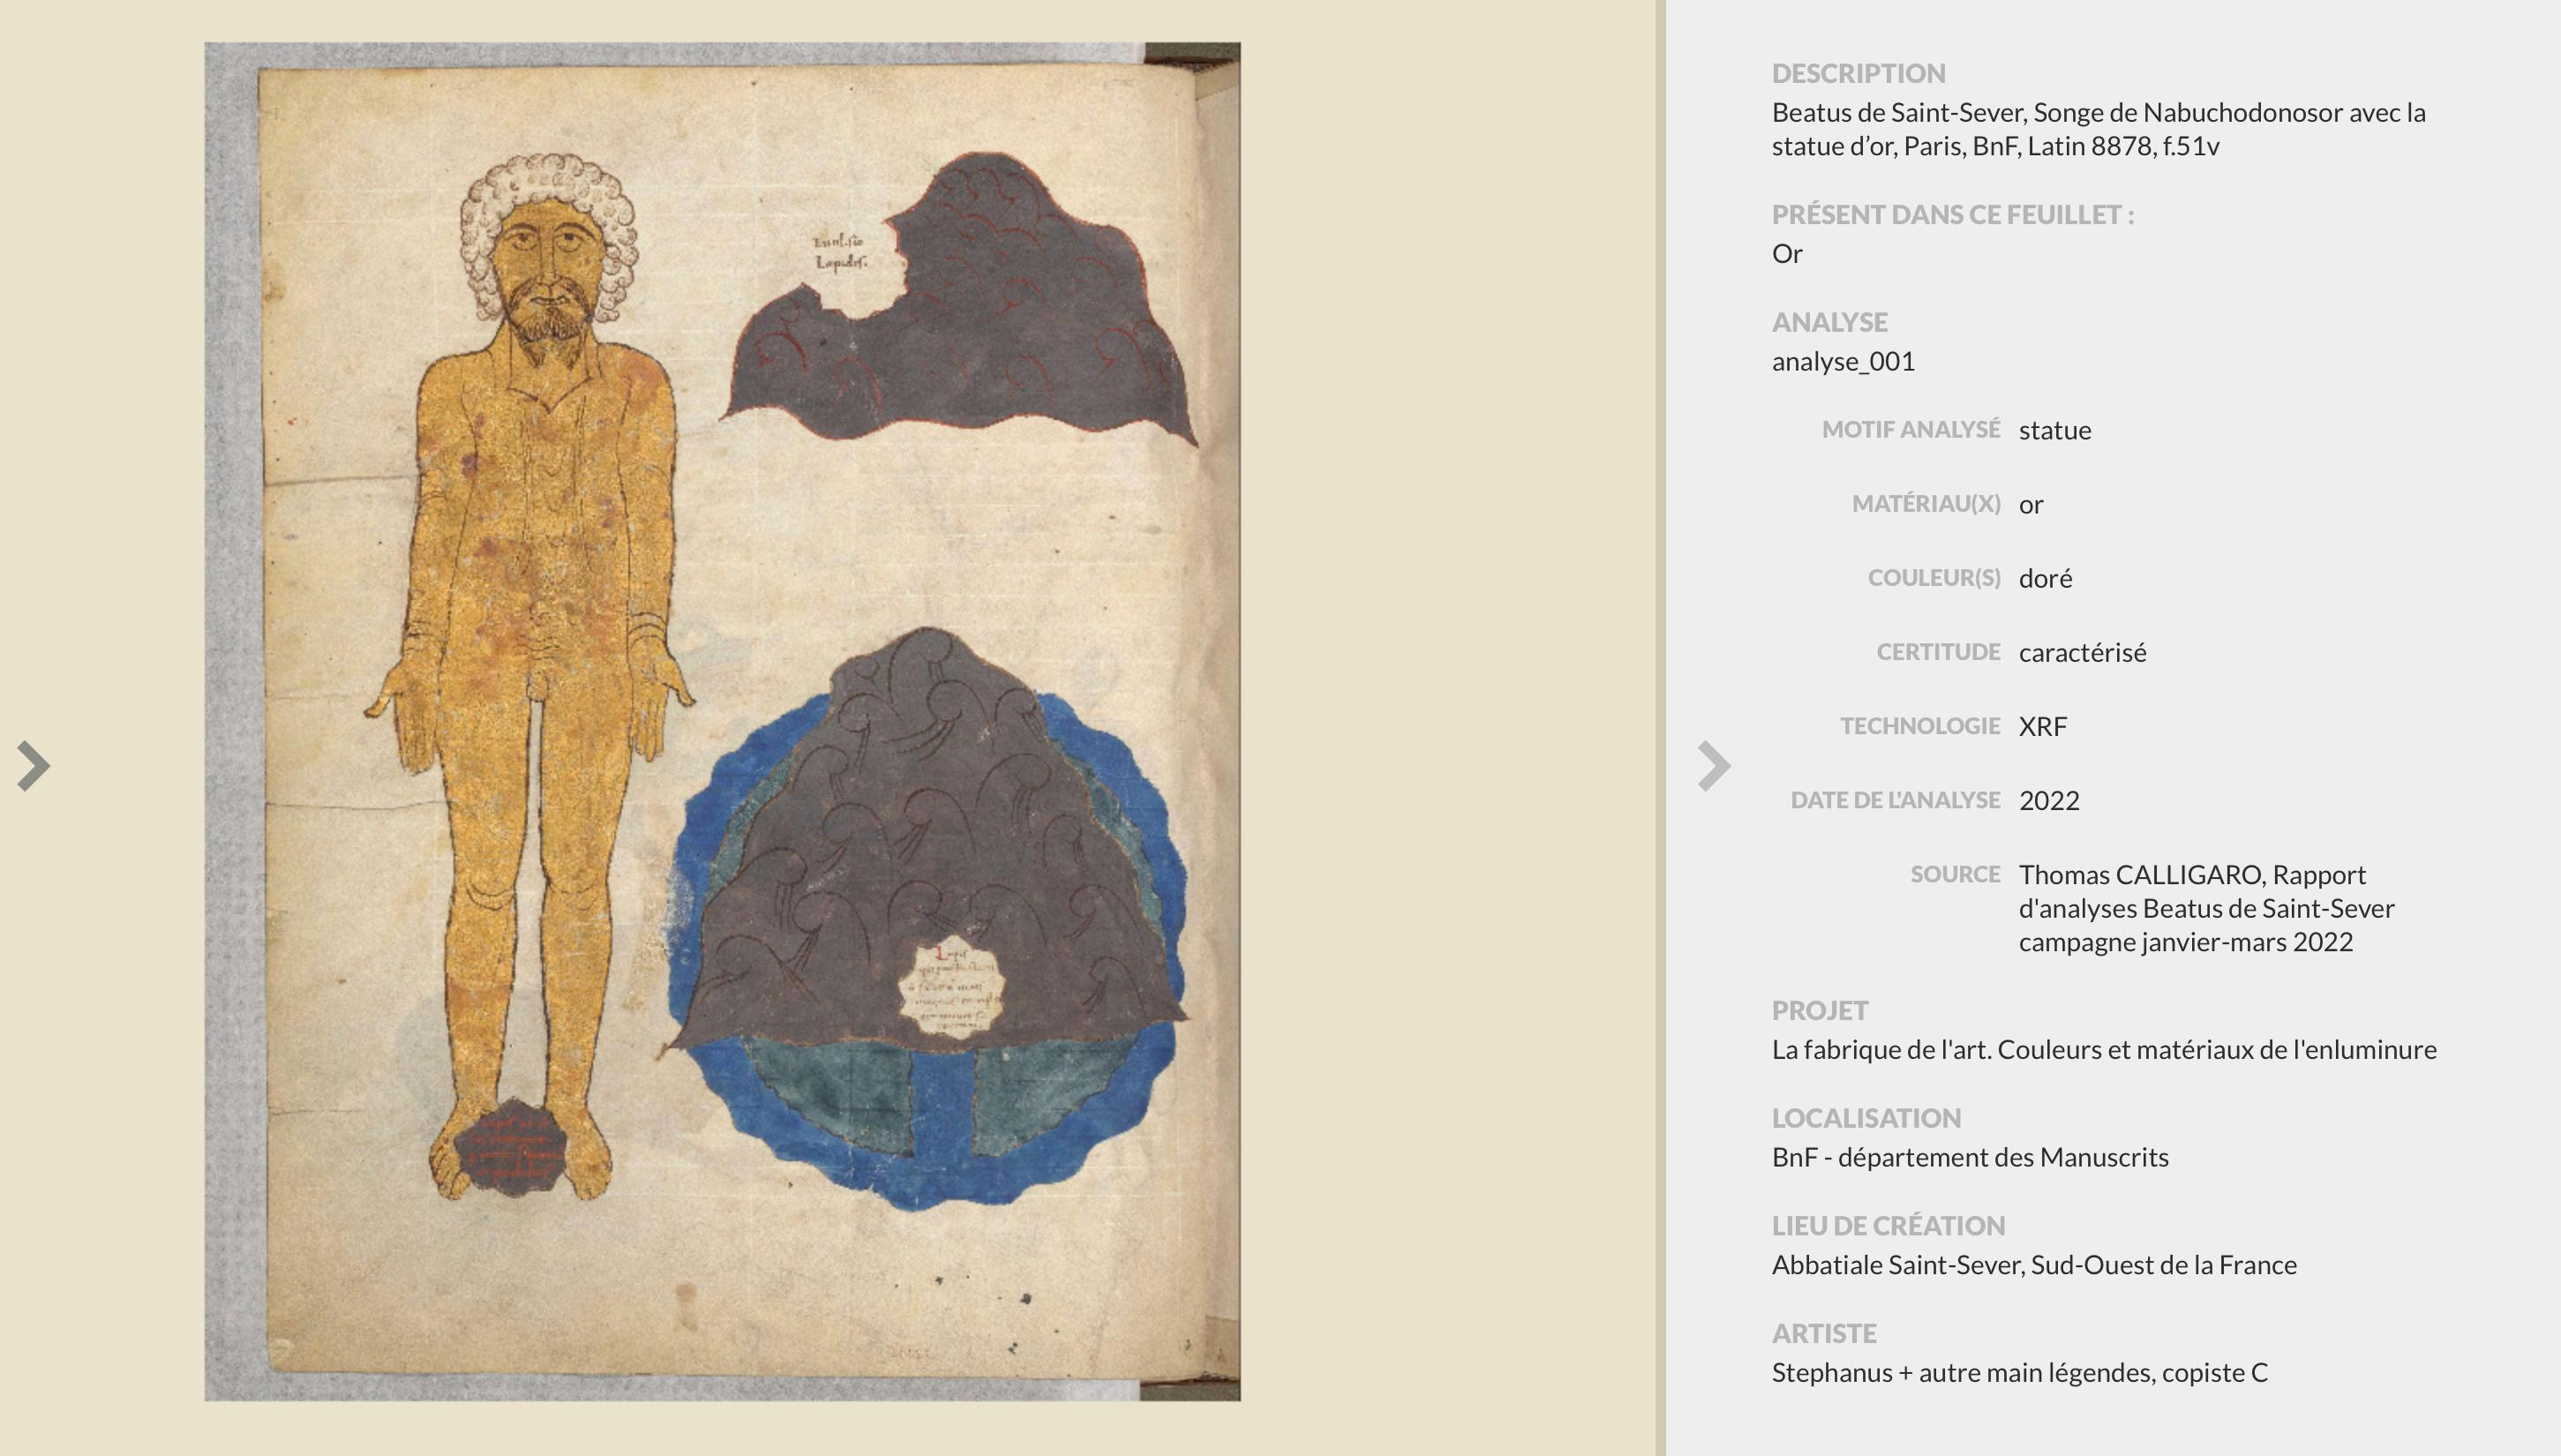
\includegraphics[width=\textwidth]{./textes/chap3/vikus-barre.jpg}
	\caption{Présentation des données sous Vikus}
	\label{fig:info}
\end{figure}

\indexmot{VIKUS} Viewer permet de travailler à partir de toutes les données entrées dans les deux bases du projet, materiality88 et 89. Celles-ci sont accessibles dans le champ supérieur de la fenêtre, qui permet la recherche en texte libre, que ce soit par le nom du manuscrit, de la couleur, du lieu de création ou de toute autre information. Si la \indexmot{visualisation} nécessite un certain appauvrissement de la \indexmot{chronologie}, toutes les autres données peuvent être encodées et reportées sans difficulté. Comme pour la cartographie interactive, l’essentiel de la transformation repose sur le langage Python.\newpage

\section{Traitement des données}

La \indexmot{visualisation} repose sur un fichier HTML qui est relié à des dossiers contenant du code JavaScript et du CSS\footnote{Le clonage du dépôt GitHub inclut également un dossier \enquote{font} pour les polices et un \enquote{image} pour les icônes utiles pour la mise en page.}. À cette architecture, il faut produire et ajouter un dossier \enquote{data}, qui est lu par les codes JavaScript et qui contient toutes les données qui sont traitées. La réalisation du dossier \enquote{data}, nous l’avons vu, se fait essentiellement à partir d’une imitation des exemples proposés. Dans le cas présent, je me suis inspiré du modèle réalisé pour les peintures de Van Gogh.\\\par 
Le travail repose sur la création de quatre fichiers de métadonnées qui décrivent la collection et les objets, et qui configurent la \indexmot{visualisation}. Il convient d’ajouter à ces fichiers une collection d’images, qui représentent les artefacts. Le premier fichier se nomme config.json. Il s'agit du fichier de configuration qui définit le nom du projet, les lien de données, les colonnes des artefacts, les styles et le contenu de la barre latérale qui détaille la collection.\par
Le data.csv contient toutes les informations de métadonnées pour chaque objet de la collection. Il a des champs obligatoires qui permettent de faire le lien avec les autres données. Les lignes doivent contenir au moins un identifiant, un mot-clef et une année. L’identifiant doit correspondre au nom de l’image qui sera produite par la suite. Par exemple, dans notre cas, l’identifiant fd106807-3864-4227-87ef-1ff82988616d correspond à l’image des \textit{Épîtres de saint Paul} (lettre ornée, Paris, BnF, Latin 10440, f.20r, f.20v). La complexité de l’identifiant peut surprendre, mais elle correspond en réalité à une simplification des données. Pour la préparation du fichier data.csv, je m’appuie sur le fichier préparé pour la cartographie. Afin de faire apparaître les résultats par feuillets, et non par analyses, je réalise un pivot de ces dernières sur chaque première ligne des feuillets, tout en les ordonnant selon une nouvelle numérotation. Ensuite, il suffit de procéder à un téléchargement des images en leur assignant le numéro de l’identifiant comme nom. En ce qui concerne les mots-clés, qui portent sur les matériaux, une concaténation des différentes analyses des feuillets, toutes présentes maintenant sur les mêmes lignes, permet de constituer la colonne. Il convient de réaliser un nettoyage des entrées ensuite, afin qu’elles puissent être correctement reconnues par le code JavaScript. Ensuite, la colonne ‘year’, elle aussi obligatoire, correspond à l’approximation par demi-siècle que je dois réaliser afin de proposer une \indexmot{visualisation} intelligible. Les autres colonnes du fichier data.csv correspondent à différents champs de métadonnées qui peuvent être personnalisés. Ici, nous retrouvons les informations qui correspondent au titre du feuillet, aux différentes analyses, aux lieu de création et de conservation, ainsi qu’au projet de recherche auquel il se rattache.\par
Le timeline.csv contient les informations pour la \indexmot{chronologie} affichée sous les années. Si l’année peut être un nombre ou une chaîne de caractère, elle correspond ici aux demi-siècles de la colonne ‘year’. Ensuite, le fichier doit contenir d’autres renseignements~: un titre de présentation sous les séquences chronologiques, un texte détaillé lorsqu’il y a un premier niveau de zoom, puis un texte supplémentaire lorsqu’il est zoomé au maximum. Ces éléments doivent contribuer à fournir un contexte historique à l’utilisateur lors de son exploration de la base. Cependant, avec une \indexmot{chronologie} \textit{artificielle} comme la nôtre, il n’est pas évident d’apporter des compléments d’informations sous les séquences chronologiques. J’ai simplement opté pour le fait de mettre en toutes lettres la période considéré~; ainsi la colonne \textit{0951-1000} est accompagnée de la précision \textit{Seconde moitié du Xe siècle}.\par
Enfin, le dernier fichier de métadonnées, info.md concerne les informations affichées sur le côté gauche lors de l'ouverture de la \indexmot{visualisation}. D’une écriture simple en Markdown, j’y fais apparaître une présentation simple et concise du projet de recherche et de la prise en main de l’interface.\\\par
À côté de ces quatre fichiers, la \indexmot{visualisation} repose sur la préparation et la configuration d’une collection d’images. Ces dernières doivent être téléchargées dans un seul dossier et nommées selon l’identifiant qui leur est assigné dans le fichier data.csv. Le traitement consiste en l’application du script vikus-viewer qui génère des sprites et des textures pour les différents niveaux de zoom.\par
En premier lieu, il faut cloner le dépôt et installer les dépendances~:\par
git clone https://github.com/cpietsch/vikus-viewer-script
cd vikus-viewer-script\par
npm install\\\par
Ensuite, le script est exécuté pour générer les textures et les sprites~:\par
vikus-viewer-script \enquote{/chemin/vers/les/images/*.+(jpg|jpeg|png)}\\\par
Le script crée un dossier de données pour les textures (1024 et 4096) ainsi qu'un dossier de sprites pour les spritesheets à l'intérieur du dossier actuel. \\\par
Les créations doivent être copiées à l’intérieur du dossier data, à côté des autres fichiers présentés précédemment.\par
Une fois que tous les liens sont bien vérifiés dans le config.json, il est possible de débuter la \indexmot{visualisation} avec un serveur web sur le fichier index.html.\newpage

\section{Chronologie et interprétation}

L'un des principaux avantages de l'utilisation de la \indexmot{chronologie} est qu'elle permet aux utilisateurs de comprendre les objets dans leur contexte historique. Les manuscrits sont, dans le cas présent, ordonnancés selon l’époque à laquelle ils ont été créés. La \indexmot{géographie}, les sujets iconographiques, les artistes et mêmes les couleurs ne jouent ici aucun rôle dans le classement. C’est une distribution temporelle stricte. Il s’agit, avec \indexmot{VIKUS}, de donner la primauté à une analyse historique du corpus. Nous pouvons en proposer quelques exemples.\par
Si nous revenons au cas de notre \indexmot{bleu égyptien} déjà évoqué au cours de ce mémoire, la \indexmot{frise chronologique} fait apparaître trois séquences à son utilisation dans les enluminures. La première est datée de la seconde moitié du VIe siècle, avec le \textit{Pentateuque dit d’Ashburnham}. Une deuxième séquence est très circonstanciée à la fin du VIIIe siècle, dans l’\textit{Évangéliaire de Charlemagne}. Sa dernière apparition est au XIe siècle, principalement dans le \textit{\indexmot{Beatus de Saint-Sever}}. Ces trois temps apparaissent sur la frise, sans qu’ils soient rapportés à d’autres variables que la date de réalisation et le matériau. La \indexmot{chronologie}, plus que toute autre forme de \indexmot{visualisation}, permet de représenter les discontinuités temporelles de l’emploi du \indexmot{bleu égyptien}. Les interruptions et les reprises successives dans l’utilisation du matériau apparaissent et invitent le chercheur à s’interroger sur les raisons artistiques, culturelles et matérielles de ces retours et disparitions au cours du temps.\par

\begin{figure}[H]
	\centering
	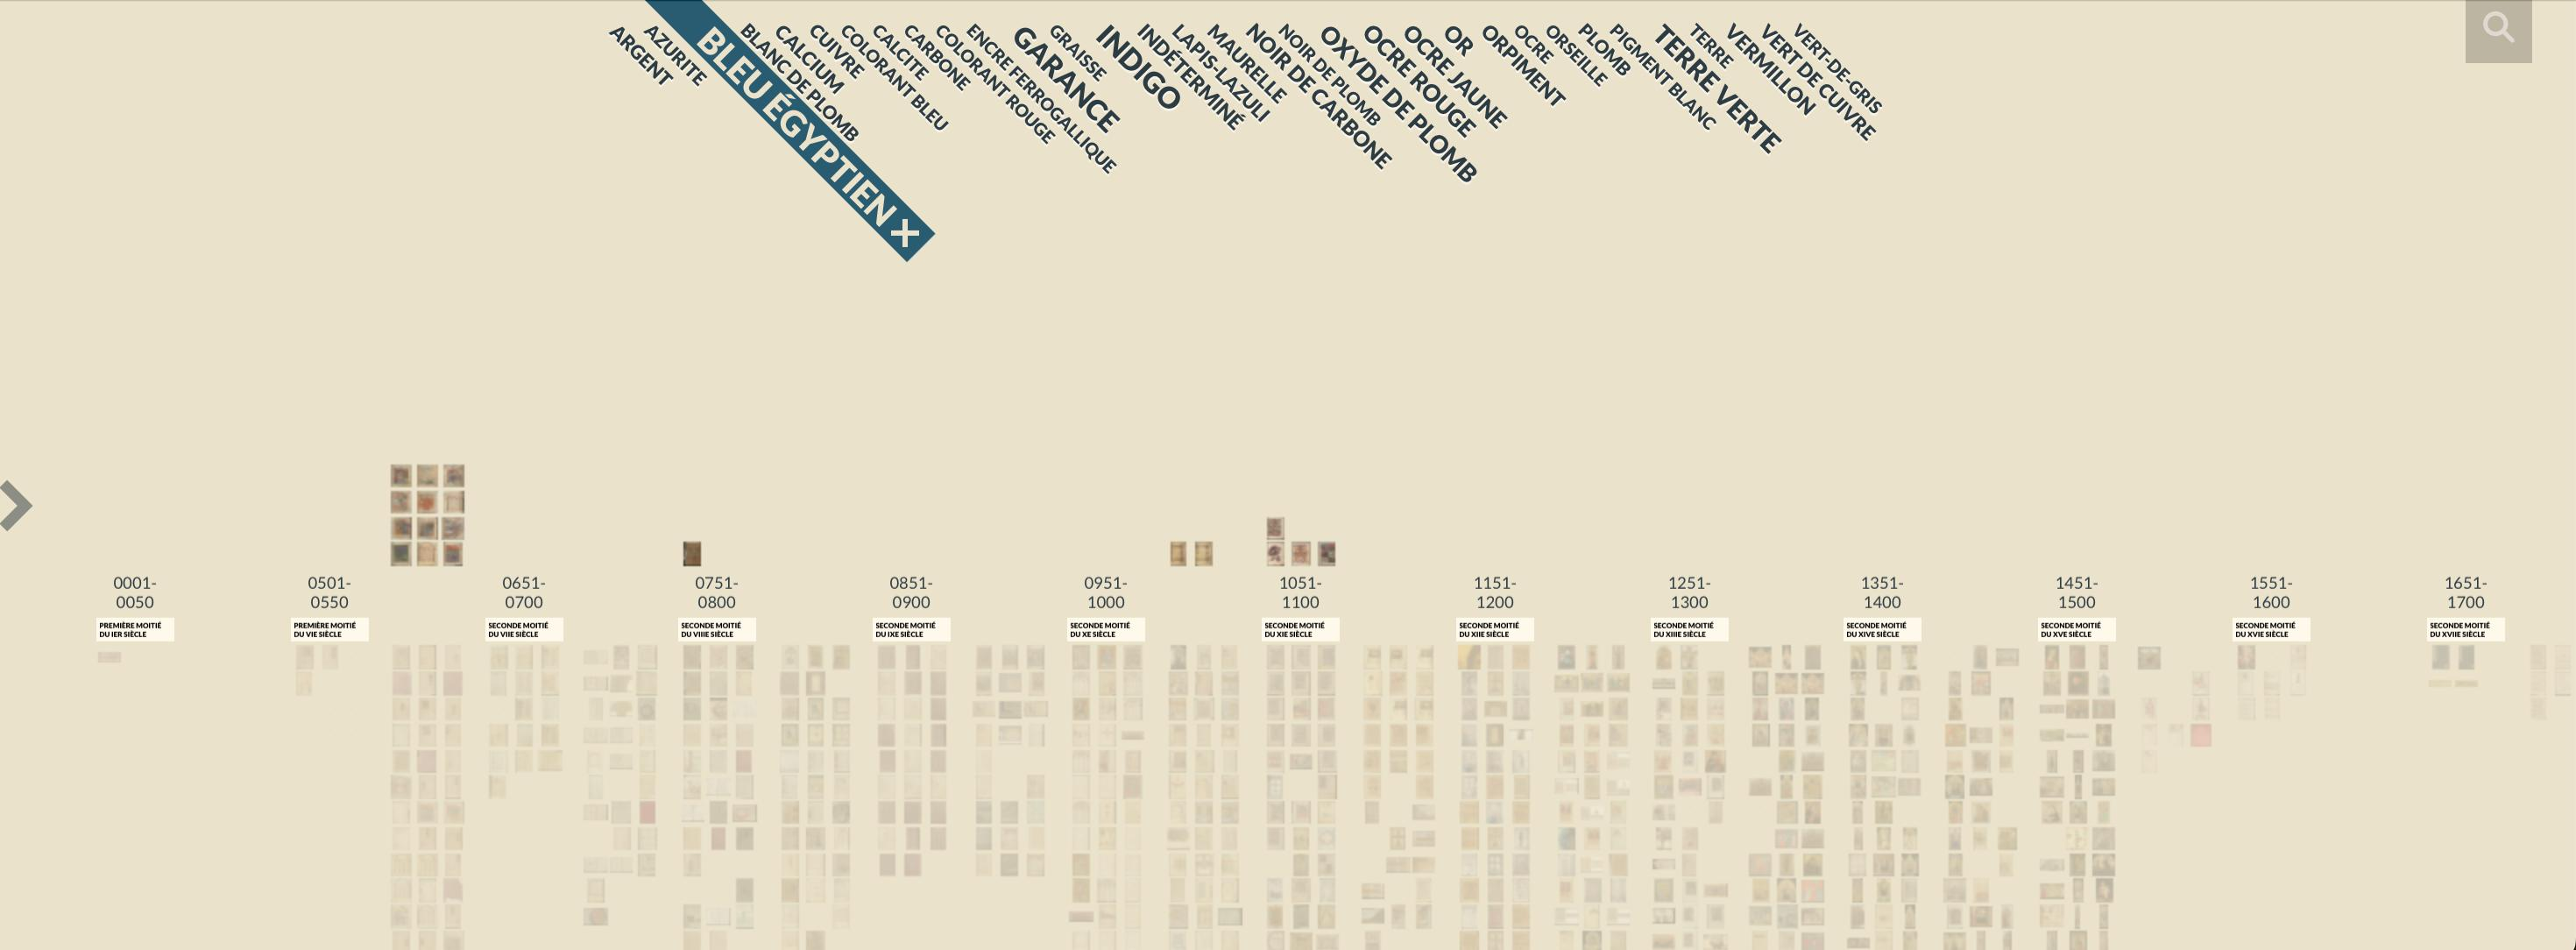
\includegraphics[width=\textwidth]{./textes/chap3/vikus-bleu-egy.jpg}
	\caption{Distribution temporelle du bleu égyptien}
	\label{fig:info}
\end{figure}

La \indexmot{chronologie} permet d'observer les évolutions et les tendances au fil du temps. Le deuxième exemple se sert de la recherche en texte libre que propose \indexmot{VIKUS} viewer pour porter un regard sur les contextes de production des enluminures. Ce champ permet d’interroger l’ensemble des données du fichier data.csv construit précédemment. En visualisant les occurrences du mot \textit{abbaye}, le résultat fait apparaître une longue séquence chronologique allant du VIIe siècle au XIe, avec une petite reprise aux alentours de l’année 1400. Une première hypothèque qui pourrait être formulée est celle de la mise en évidence, par la \indexmot{chronologie}, d’un déplacement dans le contexte de production du corpus analysé. Je n’évoque qu’une hypothèse, la base de données n’étant pas suffisamment fournie pour parvenir à une conclusion, mais la \indexmot{visualisation} invite à porter notre regard vers d’autres collections, afin de constater une même délocalisation de la production artistique, une même sortie des abbayes vers le monde.\par
La \indexmot{visualisation} reproduite ci-dessous rappelle que la \indexmot{chronologie} est aussi un discours sur le temps\footcite{toubkis_ordre_2004}. Les séquences de production des enluminures que nous avons définies, par demi-siècle, renvoie peut-être trop la \indexmot{chronologie} à un instrument taxinomique\footcite{certeau_ecriture_1975}. Avec une étude plus poussée des contextes de production de ces enluminures, il serait alors possible de proposer des \indexmot{chronologie}s-typologies sur \indexmot{VIKUS}, comme des emboîtements thématisés. Serait-il dès lors possible de recomposer un récit temporel et de concevoir comme séquence chronologique un \textit{temps de production abbatiale} par exemple?\par

\begin{figure}[H]
	\centering
	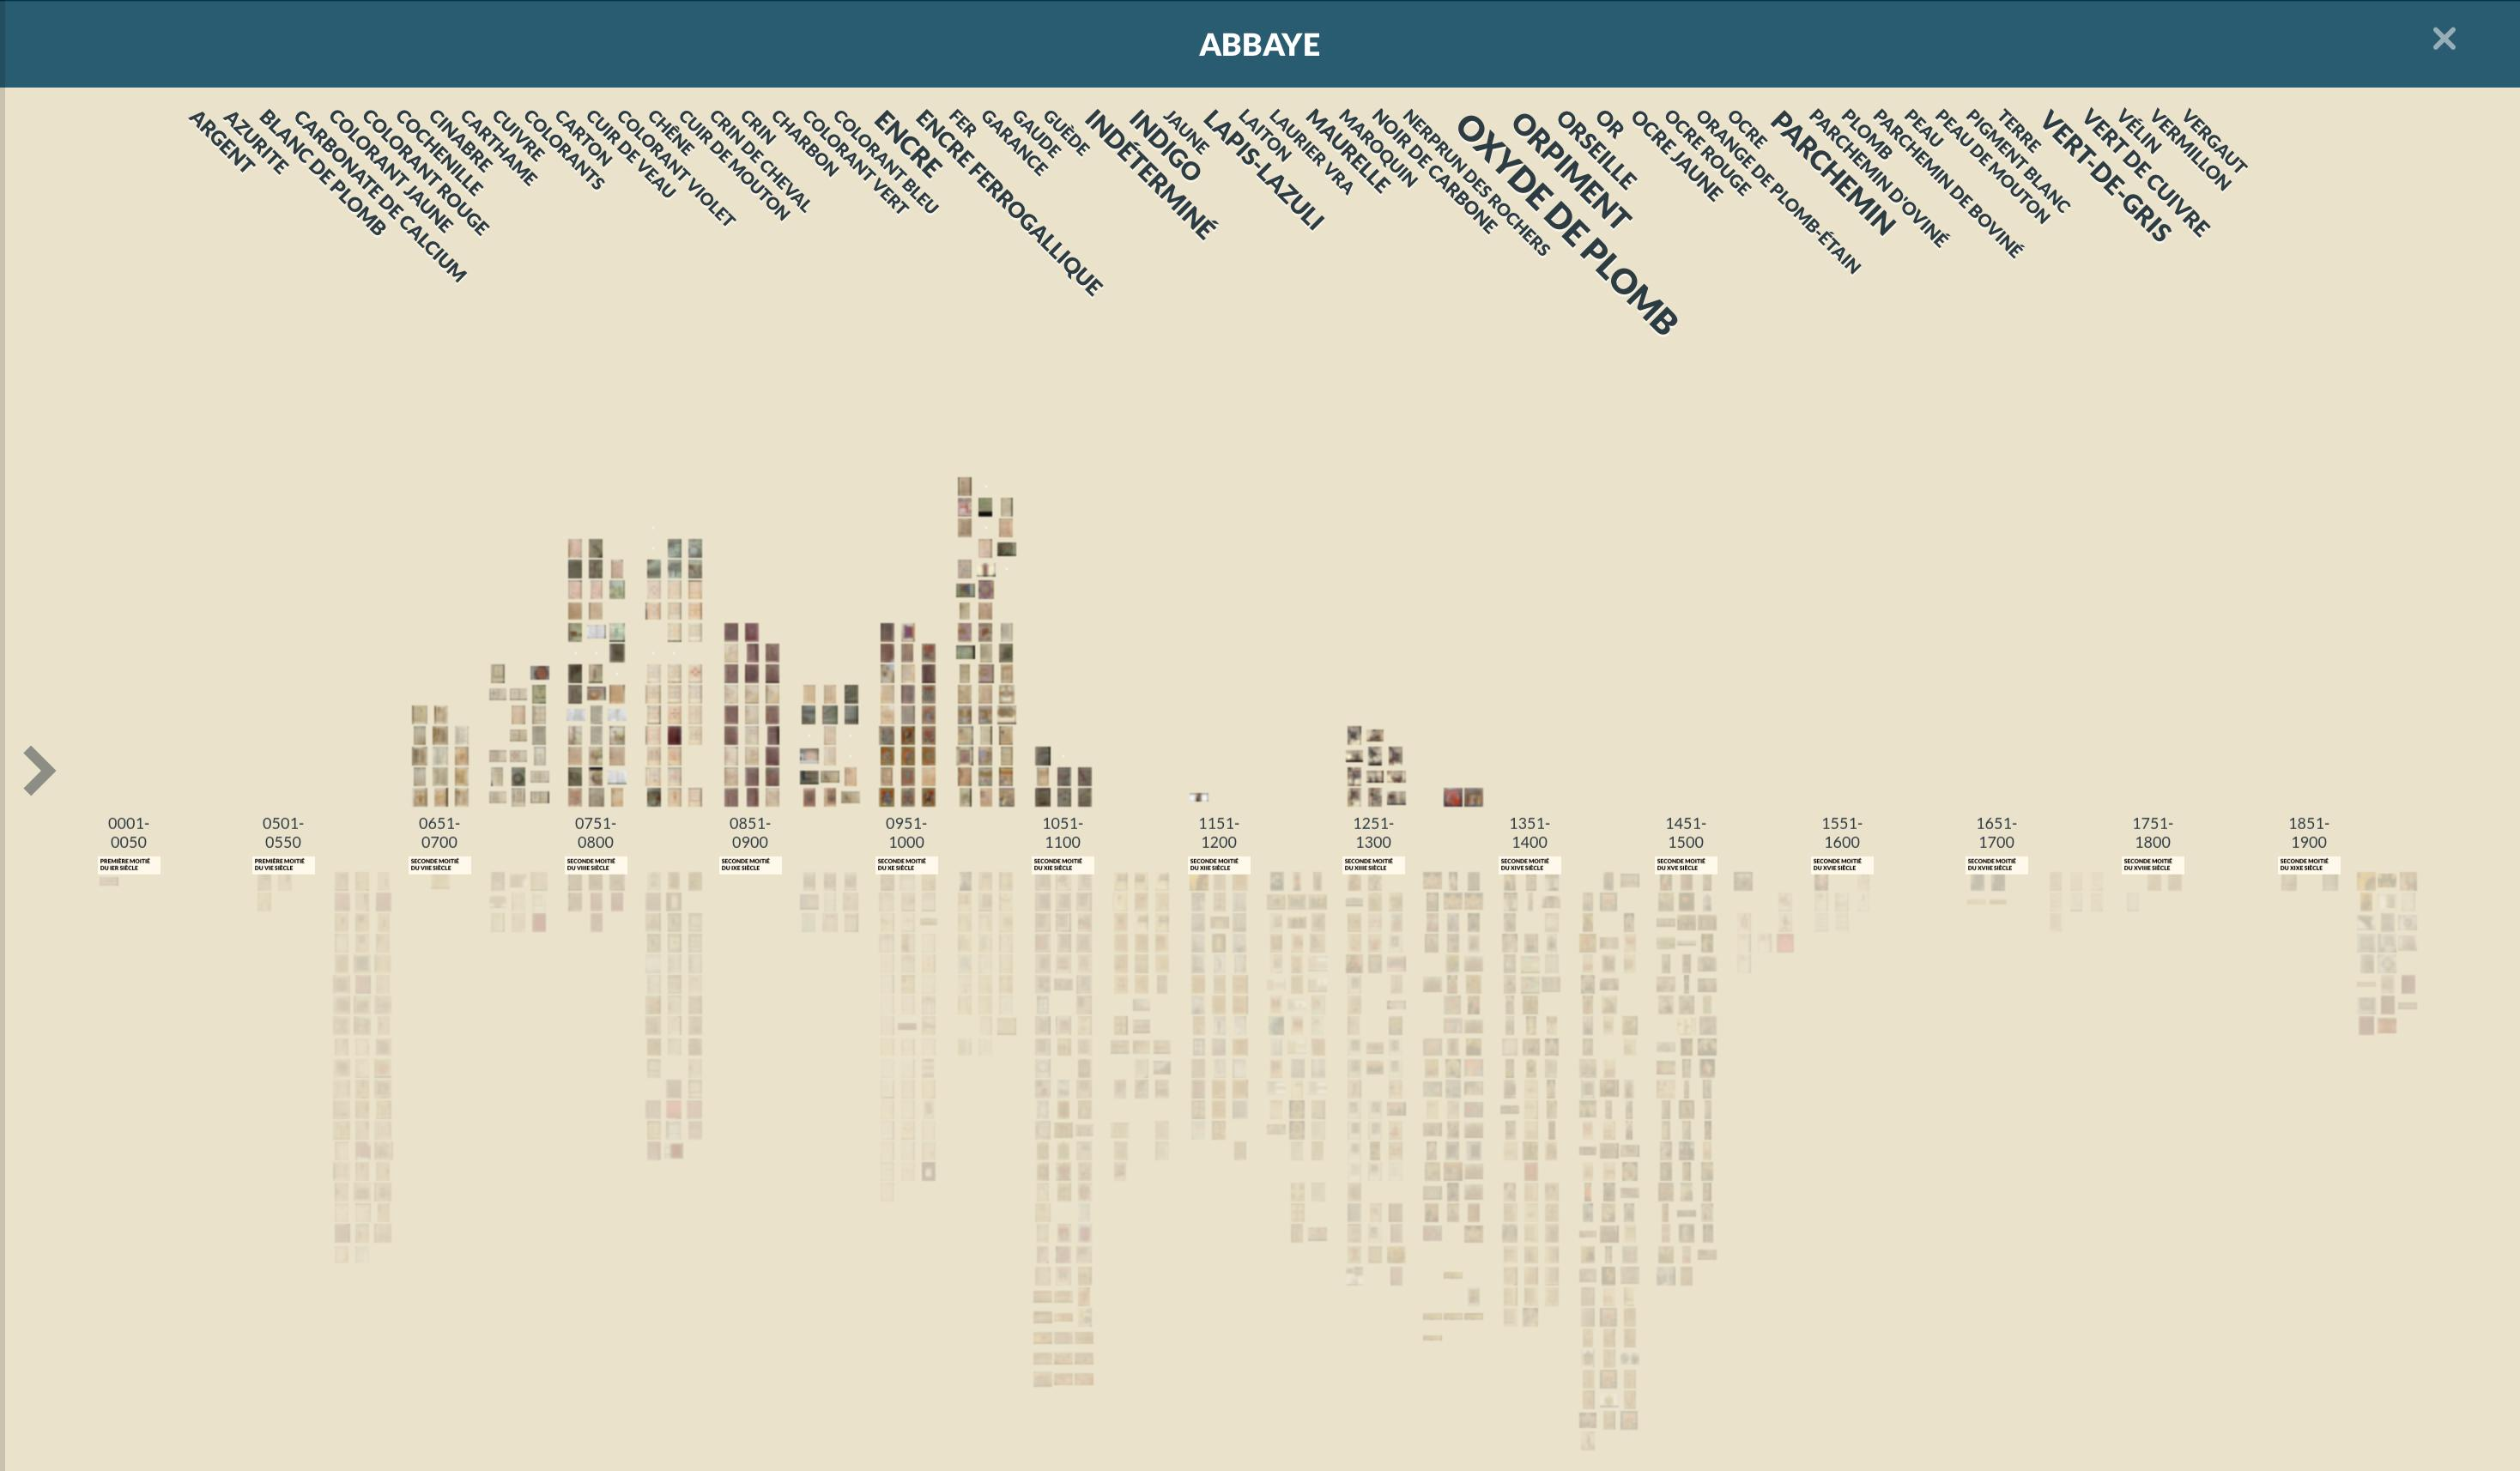
\includegraphics[width=\textwidth]{./textes/chap3/vikus-abbaye.jpg}
	\caption{Chronologie de la production abbatiale}
	\label{fig:info}
\end{figure}

\newpage
*\\\par
Ces exemples sont des parfaites illustrations des vertus heuristiques de certaines formes de \indexmot{visualisation} évoquées au cours de ce mémoire. Le brassage des données, selon des critères tantôt géographiques, tantôt chronologiques, permet l’observation de disjonctions et de continuités. Ces observations sont à la source de nouvelles analyses pour les chercheurs. \par
En somme, l'utilisation d'une \indexmot{chronologie} enrichie par des mots-clés, à l’image de celle proposée par \indexmot{VIKUS} Viewer, permet une exploration plus approfondie et contextuelle des données de la recherche. Elle offre une compréhension temporelle du corpus, elle met en lumière les évolutions et les tendances historiques, et elle facilite la comparaison selon des thèmes au fil du temps, ce qui peut être particulièrement précieux pour les chercheurs, les historiens et le grand public.

